% !TEX spellcheck = en_US



% ~~~~~~~~~~~~~~~~~~~~~~~~~~~~~~~~~~~~~~~ V
% (NC) 2026 Haluk Bingol
% github.com/halukbingol/LaTeX-Templates
%
% Licensees may copy, distribute, display, and perform the work and make derivative works 
% and remixes based on it only for non-commercial purposes. 
% ~~~~~~~~~~~~~~~~~~~~~~~~~~~~~~~~~~~~~~~ A




% =====================================================================
%  Internationalization in Java -- The Concepts
%  ---------------------------------------------------------------------
%  Built on Template/hblibTemplate.tex with the libraries in ../../hblib/.
%  Programs, terminal sessions and their real outputs are in codeoutput/:
%     codeoutput/<Name>.java  a program        codeoutput/<Name>.sh   a session
%     codeoutput/<Name>/      the session's project folder
%     codeoutput/<Name>.txt   what it printed, made by:  bash run_examples.sh
% =====================================================================

\documentclass[aspectratio=169,10pt,compress]{beamer}

% ~~~~~~~~~~~~~~~~~~~~~~~~~~~~~~~~~~~~~~~~~~~~~~~~~~~~~~~~~~~~~~~~~ V hblib
	\usepackage{../../hblib/hblibPresentation} % lib presentation: theme, i/N, \hSection, algorithm2e, ...
	\usepackage{../../hblib/hblibCodeoutput} % lib code + output: \lstcode, \lstterminal, ...
	\usepackage{../../hblib/hblibDatastructures} % lib data structures: \hString, \hStack, \hQueue
% ~~~~~~~~~~~~~~~~~~~~~~~~~~~~~~~~~~~~~~~~~~~~~~~~~~~~~~~~~~~~~~~~~ A hblib


% xcolor, array (and the L{width} column), listings, tikz and algorithm2e come from the hblib libraries
\usepackage[T1]{fontenc}
\usepackage{lmodern}
\usepackage{booktabs}

\definecolor{gitred}{RGB}{240,80,50}
\newcommand{\win}{\textbf{Windows}}
\newcommand{\mac}{\textbf{macOS}}

% algorithm2e set-up (the package is loaded by hblibPresentation), as in the template
\SetAlCapFnt{\small}
\SetAlCapNameFnt{\small}
\DontPrintSemicolon

% ---------------------------------------------------------------------
\title{Internationalization in Java}
\subtitle{The Concepts}
\author[Bingol]{Haluk O. Bingol}

\institute[FCIS]{
    Faculty of Computer and Information Sciences\\
    Yeditepe University
}
\date{
	{\tiny \hbTimeStamp}
}

\begin{document}




% ~~~~~~~~~~~~~~~~~~~~~~~~~~~~~~~~~~~~~~ V frm
\begin{frame}[t,fragile]
  \titlepage
\end{frame}
% ~~~~~~~~~~~~~~~~~~~~~~~~~~~~~~~~~~~~~~ A frm




% ~~~~~~~~~~~~~~~~~~~~~~~~~~~~~~~~~~~~~~ V frm
\begin{frame}[t,fragile] \frametitle{Outline}
  \begin{columns}[T]
    \begin{column}{0.48\textwidth}
      \tableofcontents[sections={1-4}, hideallsubsections]
    \end{column}
    \begin{column}{0.48\textwidth}
      \tableofcontents[sections={5-20}, hideallsubsections]
    \end{column}
  \end{columns}
\end{frame}
% ~~~~~~~~~~~~~~~~~~~~~~~~~~~~~~~~~~~~~~ A frm

% ~~~~~~~~~~~~~~~~~~~~~~~~~~~~~~~~~~~~~~ V
\hSection[Why]{Why Internationalization?}
% ~~~~~~~~~~~~~~~~~~~~~~~~~~~~~~~~~~~~~~ A

% ~~~~~~~~~~~~~~~~~~~~~~~~~~~~~~~~~~~~~~ V
\subsection[Problem]{One program, many users}
% ~~~~~~~~~~~~~~~~~~~~~~~~~~~~~~~~~~~~~~ A




% ~~~~~~~~~~~~~~~~~~~~~~~~~~~~~~~~~~~~~~ V frm
\begin{frame}[t,fragile] \frametitle{The same numbers, five countries}
  \lstterminal[basicstyle=\ttfamily\scriptsize]{codeoutput/SameValue.txt}
  \vspace{0.2em}
  \begin{itemize}\small
    \item The \textbf{data} is the same: $1234567.891$, $1234.5$, $0.25$, 15 October 2026.
    \item The \textbf{presentation} differs: decimal point or comma, grouping with
      \texttt{,} \texttt{.} space or \texttt{'}, symbol before or after, \%25 in Turkish, word order of dates.
    \item A program that hard-codes \texttt{"\%.2f"} or \texttt{"MM/dd/yyyy"} is right in one country and wrong in the others.
  \end{itemize}
\end{frame}
% ~~~~~~~~~~~~~~~~~~~~~~~~~~~~~~~~~~~~~~ A frm




% ~~~~~~~~~~~~~~~~~~~~~~~~~~~~~~~~~~~~~~ V frm
\begin{frame}[t,fragile] \frametitle{Three words: i18n, l10n, g11n}
  \begin{columns}[T]
    \begin{column}{0.55\textwidth}
      \begin{description}\small
        \item[i18n] \textbf{internationalization}: design the program so that it \emph{can} be adapted
          to any language and region \emph{without changing the code}. Done once, by developers.
        \item[l10n] \textbf{localization}: adapt it to \emph{one} locale: translate texts, choose formats,
          pictures, colors. Done for every new market, often by translators.
        \item[g11n] \textbf{globalization}: both together, plus the business side.
      \end{description}
      \small The numbers count the letters left out: i\,\underline{nternationalizatio}\,n has 18.
    \end{column}
    \begin{column}{0.41\textwidth}
      \begin{block}{Rule of thumb}
        \small
        i18n is an \textbf{engineering} task: separate what varies from the code.\\[0.3em]
        l10n is a \textbf{content} task: fill in the varying part for one place.
      \end{block}
      \begin{block}{Cost}
        \small Adding i18n later means touching every string and every \texttt{format} call.
        Adding it from the start costs almost nothing.
      \end{block}
    \end{column}
  \end{columns}
\end{frame}
% ~~~~~~~~~~~~~~~~~~~~~~~~~~~~~~~~~~~~~~ A frm

% ~~~~~~~~~~~~~~~~~~~~~~~~~~~~~~~~~~~~~~ V
\subsection[What varies]{What varies}
% ~~~~~~~~~~~~~~~~~~~~~~~~~~~~~~~~~~~~~~ A




% ~~~~~~~~~~~~~~~~~~~~~~~~~~~~~~~~~~~~~~ V frm
\begin{frame}[t,fragile] \frametitle{What changes from one culture to another}
  \begin{center}\scriptsize
  \begin{tabular}{L{0.2\textwidth}L{0.34\textwidth}L{0.36\textwidth}}
    \toprule
    \textbf{Item} & \textbf{Example differences} & \textbf{Java} \\
    \midrule
    texts           & ``Save'', ``Kaydet'', ``Speichern''            & \texttt{ResourceBundle} \\
    messages        & word order, plural forms                       & \texttt{MessageFormat} \\
    numbers         & \texttt{1,234.5} \quad \texttt{1.234,5} \quad \texttt{1 234,5} & \texttt{NumberFormat} \\
    currency        & \texttt{\$12.50} \quad \texttt{12,50 \texteuro} \quad \hbLira\texttt{12,50} & \texttt{NumberFormat}, \texttt{Currency} \\
    dates, times    & \texttt{10/15/26} \quad \texttt{15.10.2026}, 12 or 24 hours & \texttt{DateTimeFormatter} \\
    time zones      & UTC+3 all year in Istanbul, daylight saving elsewhere & \texttt{ZoneId}, \texttt{ZonedDateTime} \\
    calendars       & Gregorian, Buddhist, Hijri, Japanese           & \texttt{java.time.chrono} \\
    sorting         & where \texttt{ç}, \texttt{ı}, \texttt{ö} go in a list & \texttt{Collator} \\
    upper/lower case & \texttt{i}\,$\to$\,\texttt{İ} in Turkish, \texttt{ß}\,$\to$\,\texttt{SS} in German & \texttt{toUpperCase(Locale)} \\
    writing         & alphabet, direction (left-to-right, right-to-left) & \texttt{Character}, \texttt{Bidi} \\
    others          & names, addresses, phone numbers, units, paper size & application code \\
    \bottomrule
  \end{tabular}
  \end{center}
\end{frame}
% ~~~~~~~~~~~~~~~~~~~~~~~~~~~~~~~~~~~~~~ A frm

% ~~~~~~~~~~~~~~~~~~~~~~~~~~~~~~~~~~~~~~ V
\hSection[Locale]{Locales}
% ~~~~~~~~~~~~~~~~~~~~~~~~~~~~~~~~~~~~~~ A

% ~~~~~~~~~~~~~~~~~~~~~~~~~~~~~~~~~~~~~~ V
\subsection[Tags]{Language tags}
% ~~~~~~~~~~~~~~~~~~~~~~~~~~~~~~~~~~~~~~ A




% ~~~~~~~~~~~~~~~~~~~~~~~~~~~~~~~~~~~~~~ V frm
\begin{frame}[t,fragile] \frametitle{A locale names a language and a region}
  \begin{columns}[T]
    \begin{column}{0.56\textwidth}
      \begin{center}
      \begin{tikzpicture}[part/.style={draw, rounded corners, font=\ttfamily\large, minimum height=0.8cm, inner sep=4pt},
                          lab/.style={font=\scriptsize, align=center}]
        \node[part, fill=blue!10] (l) at (0,0) {sr};
        \node[font=\ttfamily\large] at (0.65,0) {-};
        \node[part, fill=orange!15] (s) at (1.5,0) {Latn};
        \node[font=\ttfamily\large] at (2.35,0) {-};
        \node[part, fill=green!12] (r) at (3.0,0) {RS};
        \node[font=\ttfamily\large] at (3.65,0) {-};
        \node[part, fill=gray!15] (e) at (4.9,0) {u-nu-latn};
        \node[lab, below=0.2cm of l] {language\\ISO 639};
        \node[lab, below=0.2cm of s] {script\\ISO 15924};
        \node[lab, below=0.2cm of r] {region\\ISO 3166};
        \node[lab, below=0.2cm of e] {extension\\(numbers: Latin)};
      \end{tikzpicture}
      \end{center}
      \small Serbian, written in the Latin alphabet, as used in Serbia.
      Only the language is required; the others are added when they matter.
    \end{column}
    \begin{column}{0.4\textwidth}
      \begin{center}\small
      \begin{tabular}{ll}
        \toprule
        \textbf{tag} & \textbf{meaning} \\
        \midrule
        \texttt{tr}     & Turkish \\
        \texttt{tr-TR}  & Turkish, Türkiye \\
        \texttt{tr-CY}  & Turkish, Cyprus \\
        \texttt{en-US}  & English, United States \\
        \texttt{en-GB}  & English, United Kingdom \\
        \texttt{de-CH}  & German, Switzerland \\
        \texttt{pt-BR}  & Portuguese, Brazil \\
        \bottomrule
      \end{tabular}
      \end{center}
      \small Standard: \textbf{BCP\,47} (IETF). Java writes \texttt{tr\_TR} in \texttt{toString()}
      and \texttt{tr-TR} in \texttt{toLanguageTag()}.
    \end{column}
  \end{columns}
\end{frame}
% ~~~~~~~~~~~~~~~~~~~~~~~~~~~~~~~~~~~~~~ A frm

% ~~~~~~~~~~~~~~~~~~~~~~~~~~~~~~~~~~~~~~ V
\subsection[Default]{The default locale}
% ~~~~~~~~~~~~~~~~~~~~~~~~~~~~~~~~~~~~~~ A




% ~~~~~~~~~~~~~~~~~~~~~~~~~~~~~~~~~~~~~~ V frm
\begin{frame}[t,fragile] \frametitle{Where does the default locale come from?}
  \begin{columns}[T]
    \begin{column}{0.5\textwidth}
      \begin{center}
      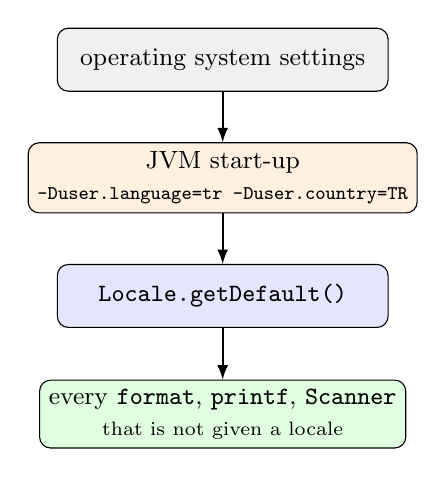
\begin{tikzpicture}[box/.style={draw, rounded corners, align=center, font=\small, minimum width=4.2cm, minimum height=0.8cm}]
        \node[box, fill=gray!12] (os) at (0,0) {operating system settings};
        \node[box, fill=orange!12] (jvm) at (0,-1.5) {JVM start-up\\\scriptsize\texttt{-Duser.language=tr -Duser.country=TR}};
        \node[box, fill=blue!10] (def) at (0,-3) {\texttt{Locale.getDefault()}};
        \node[box, fill=green!12] (fmt) at (0,-4.5) {every \texttt{format}, \texttt{printf}, \texttt{Scanner}\\\scriptsize that is not given a locale};
        \draw[-latex, thick] (os) -- (jvm);
        \draw[-latex, thick] (jvm) -- (def);
        \draw[-latex, thick] (def) -- (fmt);
      \end{tikzpicture}
      \end{center}
    \end{column}
    \begin{column}{0.46\textwidth}
      \begin{block}{\win}
        \small \menu{Settings > Time \& language > Language \& region}: \emph{Regional format}
      \end{block}
      \begin{block}{\mac}
        \small \menu{System Settings > General > Language \& Region}: \emph{Region}
      \end{block}
      \small The same program prints \texttt{3.14} on one laptop and \texttt{3,14} on the next.
      \hRemark{Programs that must give the same output everywhere pass a locale explicitly.}
    \end{column}
  \end{columns}
\end{frame}
% ~~~~~~~~~~~~~~~~~~~~~~~~~~~~~~~~~~~~~~ A frm

% ~~~~~~~~~~~~~~~~~~~~~~~~~~~~~~~~~~~~~~ V
\hSection[Text]{Characters and Encodings}
% ~~~~~~~~~~~~~~~~~~~~~~~~~~~~~~~~~~~~~~ A

% ~~~~~~~~~~~~~~~~~~~~~~~~~~~~~~~~~~~~~~ V
\subsection[Unicode]{Unicode}
% ~~~~~~~~~~~~~~~~~~~~~~~~~~~~~~~~~~~~~~ A




% ~~~~~~~~~~~~~~~~~~~~~~~~~~~~~~~~~~~~~~ V frm
\begin{frame}[t,fragile] \frametitle{Unicode: one number for every character}
  \begin{columns}[T]
    \begin{column}{0.5\textwidth}
      \begin{itemize}\small
        \item Every character has a \textbf{code point}: \texttt{A} = U+0041, \texttt{ğ} = U+011F,
          \texttt{ı} = U+0131, \texttt{\texteuro} = U+20AC, \hbLira{} = U+20BA.
        \item About 150\,000 characters: all modern scripts, symbols, emoji.
        \item An \textbf{encoding} turns code points into bytes. \textbf{UTF-8} is the standard today.
        \item Old 8-bit encodings had 256 characters: ISO-8859-9 and Windows-1254 for Turkish,
          ISO-8859-1 for Western Europe.
      \end{itemize}
    \end{column}
    \begin{column}{0.46\textwidth}
      \begin{center}\small
      \begin{tabular}{lcl}
        \toprule
        \textbf{char} & \textbf{code point} & \textbf{UTF-8 bytes} \\
        \midrule
        \texttt{A}          & U+0041  & \texttt{41} \\
        \texttt{ğ}          & U+011F  & \texttt{C4 9F} \\
        \texttt{\texteuro}  & U+20AC  & \texttt{E2 82 AC} \\
        a smiley emoji      & U+1F600 & \texttt{F0 9F 98 80} \\
        \bottomrule
      \end{tabular}
      \end{center}
      \small UTF-8 uses 1 to 4 bytes; ASCII text stays the same.
    \end{column}
  \end{columns}
\end{frame}
% ~~~~~~~~~~~~~~~~~~~~~~~~~~~~~~~~~~~~~~ A frm




% ~~~~~~~~~~~~~~~~~~~~~~~~~~~~~~~~~~~~~~ V frm
\begin{frame}[t,fragile] \frametitle{Mojibake: the wrong encoding}
  \begin{center}
  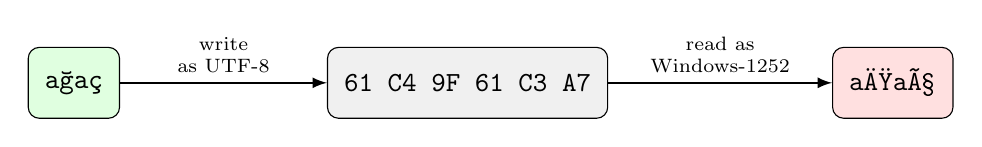
\begin{tikzpicture}[box/.style={draw, rounded corners, font=\ttfamily, minimum height=0.9cm, inner sep=6pt}]
    \node[box, fill=green!12] (a) at (0,0) {ağaç};
    \node[box, fill=gray!12] (b) at (5,0) {61 C4 9F 61 C3 A7};
    \node[box, fill=red!12] (c) at (10.4,0) {ağaç};
    \draw[-latex, thick] (a) -- node[above, font=\scriptsize, align=center] {write\\as UTF-8} (b);
    \draw[-latex, thick] (b) -- node[above, font=\scriptsize, align=center] {read as\\Windows-1252} (c);
  \end{tikzpicture}
  \end{center}
  \begin{itemize}\small
    \item The bytes are fine; the \textbf{reader} guessed the wrong encoding. This garbage is called \emph{mojibake}.
    \item Every place where text crosses a border needs an encoding: source files, \texttt{javac},
      the console, files, databases, the network.
    \item Java 18 and later use \textbf{UTF-8} by default everywhere (JEP 400). Older Java used the
      operating system's encoding, e.g.\ Windows-1254 on a Turkish Windows.
    \item Inside the program a Java \texttt{String} is a sequence of 16-bit \texttt{char}s (UTF-16);
      the encoding only matters at the borders.
  \end{itemize}
\end{frame}
% ~~~~~~~~~~~~~~~~~~~~~~~~~~~~~~~~~~~~~~ A frm

% ~~~~~~~~~~~~~~~~~~~~~~~~~~~~~~~~~~~~~~ V
\hSection[Formats]{Numbers, Money, Dates}
% ~~~~~~~~~~~~~~~~~~~~~~~~~~~~~~~~~~~~~~ A

% ~~~~~~~~~~~~~~~~~~~~~~~~~~~~~~~~~~~~~~ V
\subsection[Numbers]{Numbers and money}
% ~~~~~~~~~~~~~~~~~~~~~~~~~~~~~~~~~~~~~~ A




% ~~~~~~~~~~~~~~~~~~~~~~~~~~~~~~~~~~~~~~ V frm
\begin{frame}[t,fragile] \frametitle{Numbers and money}
  \begin{columns}[T]
    \begin{column}{0.5\textwidth}
      \begin{center}\small
      \begin{tabular}{lll}
        \toprule
        \textbf{locale} & \textbf{number} & \textbf{percent} \\
        \midrule
        \texttt{en-US} & \texttt{1,234.5}  & \texttt{25\%} \\
        \texttt{tr-TR} & \texttt{1.234,5}  & \texttt{\%25} \\
        \texttt{de-DE} & \texttt{1.234,5}  & \texttt{25 \%} \\
        \texttt{fr-FR} & \texttt{1\,234,5} & \texttt{25 \%} \\
        \texttt{de-CH} & \texttt{1'234.5}  & \texttt{25\%} \\
        \bottomrule
      \end{tabular}
      \end{center}
      \small \textbf{Parsing} has the same problem: \texttt{"1.234"} is one thousand two hundred thirty-four in
      Türkiye and one point two three four in the USA.
    \end{column}
    \begin{column}{0.46\textwidth}
      \begin{block}{Currency is two things}
        \small
        \begin{itemize}
          \item the \textbf{currency}: TRY, EUR, USD, JPY (ISO 4217), with its own number of decimals
            (JPY has none);
          \item the \textbf{format}, which follows the user's locale: a German reads
            \texttt{12,50 \$}, an American \texttt{\$12.50}.
        \end{itemize}
        Never convert money with \texttt{double}; use \texttt{BigDecimal}.
      \end{block}
    \end{column}
  \end{columns}
\end{frame}
% ~~~~~~~~~~~~~~~~~~~~~~~~~~~~~~~~~~~~~~ A frm

% ~~~~~~~~~~~~~~~~~~~~~~~~~~~~~~~~~~~~~~ V
\subsection[Time]{Dates, times, zones}
% ~~~~~~~~~~~~~~~~~~~~~~~~~~~~~~~~~~~~~~ A




% ~~~~~~~~~~~~~~~~~~~~~~~~~~~~~~~~~~~~~~ V frm
\begin{frame}[t,fragile] \frametitle{Dates, times and time zones}
  \begin{columns}[T]
    \begin{column}{0.48\textwidth}
      \textbf{Format}
      \begin{itemize}\small
        \item order: \texttt{10/15/26} (US), \texttt{15.10.2026} (TR, DE), \texttt{2026-10-15} (ISO 8601)
        \item names: \emph{Thursday}, \emph{Perşembe}, \emph{Donnerstag}
        \item clock: \texttt{2:30 PM} or \texttt{14:30}
        \item calendar: 2026 (Gregorian) is 2569 in the Thai Buddhist calendar
      \end{itemize}
      \small Store and exchange dates in \textbf{ISO 8601}; localize only for display.
    \end{column}
    \begin{column}{0.48\textwidth}
      \textbf{Time zones}
      \begin{itemize}\small
        \item the same moment: 14:30 in Istanbul is 13:30 in Berlin, 07:30 in New York, 20:30 in Tokyo
          (15 October 2026)
        \item zones have names like \texttt{Europe/Istanbul} (IANA database), not only offsets
        \item daylight saving time: clocks jump, some local times do not exist, others happen twice
        \item rules change by law; the JDK ships updates of the zone database
      \end{itemize}
    \end{column}
  \end{columns}
\end{frame}
% ~~~~~~~~~~~~~~~~~~~~~~~~~~~~~~~~~~~~~~ A frm

% ~~~~~~~~~~~~~~~~~~~~~~~~~~~~~~~~~~~~~~ V
\hSection[Messages]{Translating Messages}
% ~~~~~~~~~~~~~~~~~~~~~~~~~~~~~~~~~~~~~~ A

% ~~~~~~~~~~~~~~~~~~~~~~~~~~~~~~~~~~~~~~ V
\subsection[Bundles]{Resource bundles}
% ~~~~~~~~~~~~~~~~~~~~~~~~~~~~~~~~~~~~~~ A




% ~~~~~~~~~~~~~~~~~~~~~~~~~~~~~~~~~~~~~~ V frm
\begin{frame}[t,fragile] \frametitle{Keep texts out of the code}
  \begin{columns}[T]
    \begin{column}{0.46\textwidth}
      \begin{center}
      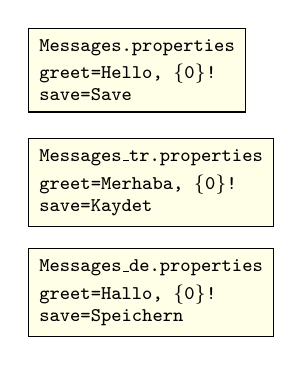
\begin{tikzpicture}[file/.style={draw, fill=yellow!10, font=\ttfamily\scriptsize, align=left, inner sep=4pt, anchor=north west}]
        \node[file] (b) at (0,0) {Messages.properties\\[2pt]greet=Hello, \{0\}!\\save=Save};
        \node[file] (t) at (0,-1.4) {Messages\_tr.properties\\[2pt]greet=Merhaba, \{0\}!\\save=Kaydet};
        \node[file] (g) at (0,-2.8) {Messages\_de.properties\\[2pt]greet=Hallo, \{0\}!\\save=Speichern};
      \end{tikzpicture}
      \end{center}
    \end{column}
    \begin{column}{0.5\textwidth}
      \begin{itemize}\small
        \item The code uses \textbf{keys}: \texttt{greet}, \texttt{save}.
        \item One file per language: a \textbf{resource bundle}. A translator edits only these files.
        \item Placeholders \texttt{\{0\}}, \texttt{\{1\}} let each language put the values where its
          grammar wants them.
        \item Adding a language = adding a file, no new code.
        \item Missing a key in \texttt{\_tr}? It is taken from the base file (\emph{fallback}).
      \end{itemize}
    \end{column}
  \end{columns}
\end{frame}
% ~~~~~~~~~~~~~~~~~~~~~~~~~~~~~~~~~~~~~~ A frm




% ~~~~~~~~~~~~~~~~~~~~~~~~~~~~~~~~~~~~~~ V frm
\begin{frame}[t,fragile] \frametitle{Finding the right file (simplified)}
% +++++++++++++++++++++++++++++++++++++++ V alg
%: -Alg. 
\begin{algorithm}[H]
  \caption{\textsc{GetBundle}$(\mathit{base}, \ell)$}
  \KwIn{base name $b$, requested locale $\ell$ (e.g.\ \texttt{tr-TR}), default locale $\delta$}
  \KwOut{a bundle whose parents form a chain down to $b$}
  $C \gets$ \textsc{Candidates}$(b, \ell)$\tcp*{\texttt{Messages\_tr\_TR}, \texttt{Messages\_tr}}
  \If{none of $C$ exists}{
    $C \gets$ \textsc{Candidates}$(b, \delta)$\tcp*{fall back to the default locale}
  }
  append $b$ to $C$\tcp*{the base file is the last resort}
  \Return{the first existing file of $C$, chained to the later ones}
\end{algorithm}
% +++++++++++++++++++++++++++++++++++++++ A alg

  \small A key is looked up in the first file, then in its parents, so a translation may be incomplete.
\end{frame}
% ~~~~~~~~~~~~~~~~~~~~~~~~~~~~~~~~~~~~~~ A frm

% ~~~~~~~~~~~~~~~~~~~~~~~~~~~~~~~~~~~~~~ V
\subsection[Grammar]{Word order and plurals}
% ~~~~~~~~~~~~~~~~~~~~~~~~~~~~~~~~~~~~~~ A




% ~~~~~~~~~~~~~~~~~~~~~~~~~~~~~~~~~~~~~~ V frm
\begin{frame}[t,fragile] \frametitle{Messages are more than words}
  \begin{columns}[T]
    \begin{column}{0.48\textwidth}
      \textbf{Word order}
      \begin{itemize}\small
        \item English: \emph{Ali sent 3 files to Ayşe.}
        \item Turkish: \emph{Ali, Ayşe'ye 3 dosya gönderdi.}
      \end{itemize}
      \small Never build sentences with \texttt{+}: \texttt{name + " sent " + n + " files"} cannot be translated.
      Use one pattern per language with numbered placeholders.
    \end{column}
    \begin{column}{0.48\textwidth}
      \textbf{Plurals}
      \begin{center}\small
      \begin{tabular}{ll}
        \toprule
        \textbf{language} & \textbf{forms after a number} \\
        \midrule
        English & 1 file, 2 files \\
        Turkish & 1 dosya, 2 dosya (noun stays singular) \\
        Polish  & 3 forms (1, 2--4, 5+) \\
        Arabic  & 6 forms \\
        \bottomrule
      \end{tabular}
      \end{center}
      \small The rules come from the Unicode CLDR project.
    \end{column}
  \end{columns}
\end{frame}
% ~~~~~~~~~~~~~~~~~~~~~~~~~~~~~~~~~~~~~~ A frm

% ~~~~~~~~~~~~~~~~~~~~~~~~~~~~~~~~~~~~~~ V
\hSection[Comparing]{Sorting and Case}
% ~~~~~~~~~~~~~~~~~~~~~~~~~~~~~~~~~~~~~~ A

% ~~~~~~~~~~~~~~~~~~~~~~~~~~~~~~~~~~~~~~ V
\subsection[Case]{The Turkish i}
% ~~~~~~~~~~~~~~~~~~~~~~~~~~~~~~~~~~~~~~ A




% ~~~~~~~~~~~~~~~~~~~~~~~~~~~~~~~~~~~~~~ V frm
\begin{frame}[t,fragile] \frametitle{Upper and lower case depend on the language}
  \begin{columns}[T]
    \begin{column}{0.5\textwidth}
      \begin{center}
      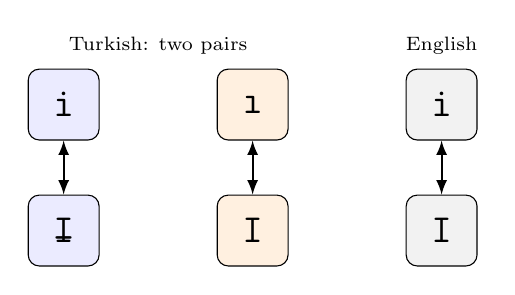
\begin{tikzpicture}[ch/.style={draw, rounded corners, font=\Large\ttfamily, minimum size=0.9cm}]
        \node[ch, fill=blue!8] (i)  at (0,0)    {i};
        \node[ch, fill=blue!8] (I1) at (0,-1.6) {İ};
        \node[ch, fill=orange!12] (di) at (2.4,0) {ı};
        \node[ch, fill=orange!12] (I2) at (2.4,-1.6) {I};
        \draw[latex-latex, thick] (i) -- (I1);
        \draw[latex-latex, thick] (di) -- (I2);
        \node[font=\scriptsize] at (1.2,0.75) {Turkish: two pairs};
        \node[ch, fill=gray!10] (ei) at (4.8,0) {i};
        \node[ch, fill=gray!10] (eI) at (4.8,-1.6) {I};
        \draw[latex-latex, thick] (ei) -- (eI);
        \node[font=\scriptsize] at (4.8,0.75) {English};
      \end{tikzpicture}
      \end{center}
      \small \texttt{"title".toUpperCase()} gives \texttt{"TİTLE"} on a Turkish computer.
    \end{column}
    \begin{column}{0.46\textwidth}
      \begin{itemize}\small
        \item Text for \textbf{people}: use the user's locale, \texttt{toUpperCase(locale)}.
        \item Text for \textbf{programs} (keywords, file names, HTTP headers, enum names):
          use \texttt{toUpperCase(Locale.ROOT)}.
        \item Famous bugs: \texttt{"FILE".toLowerCase().equals("file")} is \textbf{false} on Turkish systems;
          many libraries and tools failed this way.
        \item German \texttt{ß} becomes \texttt{SS}: the string gets longer.
      \end{itemize}
    \end{column}
  \end{columns}
\end{frame}
% ~~~~~~~~~~~~~~~~~~~~~~~~~~~~~~~~~~~~~~ A frm

% ~~~~~~~~~~~~~~~~~~~~~~~~~~~~~~~~~~~~~~ V
\subsection[Sorting]{Sorting}
% ~~~~~~~~~~~~~~~~~~~~~~~~~~~~~~~~~~~~~~ A




% ~~~~~~~~~~~~~~~~~~~~~~~~~~~~~~~~~~~~~~ V frm
\begin{frame}[t,fragile] \frametitle{Alphabetical order depends on the language}
  \begin{columns}[T]
    \begin{column}{0.48\textwidth}
      \begin{itemize}\small
        \item \texttt{String.compareTo} compares \textbf{code point numbers}: \texttt{Z} (90) $<$ \texttt{a} (97)
          $<$ \texttt{ç} (231) $<$ \texttt{ı} (305).
        \item People expect the \textbf{alphabet}: Turkish puts \texttt{ç} after \texttt{c}, \texttt{ı} before \texttt{i}.
        \item A \textbf{collator} knows the rules of one language and how strict to be
          (ignore case? ignore accents?).
      \end{itemize}
    \end{column}
    \begin{column}{0.48\textwidth}
      \begin{center}\small
      \begin{tabular}{ll}
        \toprule
        \textbf{by code point} & \textbf{Turkish alphabet} \\
        \midrule
        Ali   & ağaç \\
        araba & Ali \\
        ağaç  & araba \\
        cam   & cam \\
        ilaç  & çay \\
        Ömer  & ılık \\
        çay   & ilaç \\
        ılık  & Ömer \\
        \bottomrule
      \end{tabular}
      \end{center}
    \end{column}
  \end{columns}
\end{frame}
% ~~~~~~~~~~~~~~~~~~~~~~~~~~~~~~~~~~~~~~ A frm




% ~~~~~~~~~~~~~~~~~~~~~~~~~~~~~~~~~~~~~~ V frm
\begin{frame}[t,fragile] \frametitle{Same look, different characters: normalization}
  \begin{columns}[T]
    \begin{column}{0.5\textwidth}
      \begin{center}
      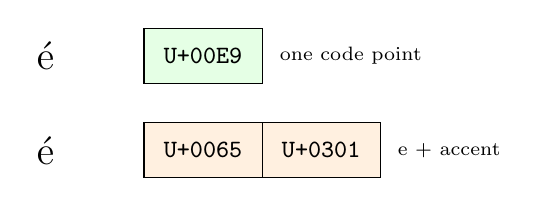
\begin{tikzpicture}[ch/.style={draw, font=\ttfamily\small, minimum width=1.5cm, minimum height=0.7cm}]
        \node[font=\Large] at (-1.4,0) {é};
        \node[ch, fill=green!10] at (0.6,0) {U+00E9};
        \node[font=\scriptsize, right] at (1.45,0) {one code point};
        \node[font=\Large] at (-1.4,-1.2) {é};
        \node[ch, fill=orange!12] at (0.6,-1.2) {U+0065};
        \node[ch, fill=orange!12] at (2.1,-1.2) {U+0301};
        \node[font=\scriptsize, right] at (2.95,-1.2) {e + accent};
      \end{tikzpicture}
      \end{center}
    \end{column}
    \begin{column}{0.46\textwidth}
      \begin{itemize}\small
        \item Both look the same, but \texttt{equals} says \textbf{false}, and \texttt{length()} is 1 or 2.
        \item Text from keyboards, files and the web can come in either form (macOS file names often use the second).
        \item \textbf{Normalize} before comparing or storing: \texttt{java.text.Normalizer}, form NFC.
      \end{itemize}
    \end{column}
  \end{columns}
\end{frame}
% ~~~~~~~~~~~~~~~~~~~~~~~~~~~~~~~~~~~~~~ A frm

% ~~~~~~~~~~~~~~~~~~~~~~~~~~~~~~~~~~~~~~ V
\hSection[Java]{The Java Toolbox}
% ~~~~~~~~~~~~~~~~~~~~~~~~~~~~~~~~~~~~~~ A




% ~~~~~~~~~~~~~~~~~~~~~~~~~~~~~~~~~~~~~~ V frm
\begin{frame}[t,fragile] \frametitle{Where to find what}
  \begin{center}\scriptsize
  \begin{tabular}{L{0.23\textwidth}L{0.33\textwidth}L{0.34\textwidth}}
    \toprule
    \textbf{task} & \textbf{class} & \textbf{package} \\
    \midrule
    name a locale         & \texttt{Locale}                        & \texttt{java.util} \\
    translated texts      & \texttt{ResourceBundle}                & \texttt{java.util} \\
    messages with values  & \texttt{MessageFormat}, \texttt{ChoiceFormat} & \texttt{java.text} \\
    numbers, money        & \texttt{NumberFormat}, \texttt{Currency}, \texttt{BigDecimal} & \texttt{java.text}, \texttt{java.util}, \texttt{java.math} \\
    dates and times       & \texttt{DateTimeFormatter}, \texttt{ZonedDateTime} & \texttt{java.time}, \texttt{java.time.format} \\
    sorting               & \texttt{Collator}                      & \texttt{java.text} \\
    normalization         & \texttt{Normalizer}                    & \texttt{java.text} \\
    words, sentences      & \texttt{BreakIterator}                 & \texttt{java.text} \\
    encodings             & \texttt{Charset}, \texttt{StandardCharsets} & \texttt{java.nio.charset} \\
    \bottomrule
  \end{tabular}
  \end{center}
  \vspace{0.3em}
  \small The locale data (names of months, formats, sorting rules) comes from the
  \textbf{Unicode CLDR} project, the default source since Java 9. Java 21 supports Unicode 15.0.
\end{frame}
% ~~~~~~~~~~~~~~~~~~~~~~~~~~~~~~~~~~~~~~ A frm

% ~~~~~~~~~~~~~~~~~~~~~~~~~~~~~~~~~~~~~~ V
\hSection[Process]{Doing It Right}
% ~~~~~~~~~~~~~~~~~~~~~~~~~~~~~~~~~~~~~~ A




% ~~~~~~~~~~~~~~~~~~~~~~~~~~~~~~~~~~~~~~ V frm
\begin{frame}[t,fragile] \frametitle{An internationalization process}
  \begin{center}
  \begin{tikzpicture}[st/.style={draw, rounded corners, fill=blue!8, align=center, font=\small, minimum width=2.4cm, minimum height=1.1cm}, node distance=0.5cm]
    \node[st] (a) {externalize\\\scriptsize texts to bundles};
    \node[st, right=of a] (b) {format\\\scriptsize with a locale};
    \node[st, right=of b] (c) {pseudo-\\localize, test};
    \node[st, right=of c, fill=orange!12] (d) {translate\\\scriptsize (l10n)};
    \node[st, right=of d, fill=green!12] (e) {test in each\\locale, ship};
    \draw[-latex, thick] (a) -- (b); \draw[-latex, thick] (b) -- (c);
    \draw[-latex, thick] (c) -- (d); \draw[-latex, thick] (d) -- (e);
    \draw[-latex, thick, dashed] (e.south) -- ++(0,-0.6) -| node[pos=0.25, below, font=\scriptsize] {a new language: only translate and test} (d.south);
  \end{tikzpicture}
  \end{center}
  \begin{itemize}\small
    \item \textbf{Pseudo-localization}: replace every text with a longer, accented version
      (\texttt{Save} $\to$ \texttt{[Šàvé !!!]}) to find hard-coded strings and too-small buttons \emph{before} translation.
    \item Leave room: German and Finnish texts are often 30\% longer than English.
    \item Test with a Turkish locale: it finds case-mapping and decimal-comma bugs quickly.
  \end{itemize}
\end{frame}
% ~~~~~~~~~~~~~~~~~~~~~~~~~~~~~~~~~~~~~~ A frm

% ~~~~~~~~~~~~~~~~~~~~~~~~~~~~~~~~~~~~~~ V
\hSection[Summary]{Summary}
% ~~~~~~~~~~~~~~~~~~~~~~~~~~~~~~~~~~~~~~ A




% ~~~~~~~~~~~~~~~~~~~~~~~~~~~~~~~~~~~~~~ V frm
\begin{frame}[t,fragile] \frametitle{Big ideas}
  \begin{itemize}
    \item i18n separates \textbf{what varies by culture} from the code; l10n fills it in for one locale.
    \item A \textbf{locale} (\texttt{tr-TR}) chooses language and conventions; the default comes from the
      operating system, so pass a locale when the output must not change.
    \item Text is \textbf{Unicode}; bytes need an \textbf{encoding}, preferably UTF-8, at every border.
    \item Numbers, money, dates, sorting and case all depend on the locale: use the Java classes, not
      hand-made patterns.
    \item Translated texts live in \textbf{resource bundles}, with placeholders, never glued with \texttt{+}.
  \end{itemize}
\end{frame}
% ~~~~~~~~~~~~~~~~~~~~~~~~~~~~~~~~~~~~~~ A frm




% ~~~~~~~~~~~~~~~~~~~~~~~~~~~~~~~~~~~~~~ V frm
\begin{frame}[t,fragile] \frametitle{Check yourself}
  \begin{enumerate}\small
    \item Why is \texttt{i18n} written with 18?
    \item What do the parts of \texttt{pt-BR} and \texttt{sr-Latn-RS} mean?
    \item A file shows \texttt{Başlık}. What went wrong, and what was the original word?
    \item Why can \texttt{"1.234"} mean two different numbers?
    \item Which locale should \texttt{toLowerCase} use for an HTTP header name? Why?
    \item Why does \texttt{Collections.sort} put \texttt{Ömer} after \texttt{zil}?
    \item Why is \texttt{"Ali sent " + n + " files"} bad for translation?
    \item Where do you change the regional format on your own computer?
  \end{enumerate}
\end{frame}
% ~~~~~~~~~~~~~~~~~~~~~~~~~~~~~~~~~~~~~~ A frm




% ~~~~~~~~~~~~~~~~~~~~~~~~~~~~~~~~~~~~~~ V frm
\begin{frame}[t,fragile]
	\begin{center}
		\vspace{4cm}
		\hRemark{\Huge Questions?}
	\end{center}
\end{frame}
% ~~~~~~~~~~~~~~~~~~~~~~~~~~~~~~~~~~~~~~ A frm



\end{document}
